\documentclass[conference,a4paper]{IEEEtran}
\usepackage[T1]{fontenc}
\usepackage[utf8]{inputenc}
\usepackage{amsmath,amssymb}
\usepackage{graphicx,booktabs,array}
\usepackage{cite}
\usepackage{xcolor}
\usepackage{url}
\usepackage[colorlinks=true,linkcolor=blue,citecolor=blue,urlcolor=blue]{hyperref}
% Generated direct-publication numeric links; bibliography stays in first-citation order.
\makeatletter
\expandafter\def\csname puburl@lewisrag\endcsname{https://arxiv.org/abs/2005.11401}
\expandafter\def\csname pubnum@lewisrag\endcsname{1}
\expandafter\def\csname puburl@ragtruth\endcsname{https://aclanthology.org/2024.acl-long.585/}
\expandafter\def\csname pubnum@ragtruth\endcsname{2}
\expandafter\def\csname puburl@maynez\endcsname{https://aclanthology.org/2020.acl-main.173/}
\expandafter\def\csname pubnum@maynez\endcsname{3}
\expandafter\def\csname puburl@halueval\endcsname{https://aclanthology.org/2023.emnlp-main.397/}
\expandafter\def\csname pubnum@halueval\endcsname{4}
\expandafter\def\csname puburl@fever\endcsname{https://aclanthology.org/N18-1074/}
\expandafter\def\csname pubnum@fever\endcsname{5}
\expandafter\def\csname puburl@scifact\endcsname{https://aclanthology.org/2020.emnlp-main.609/}
\expandafter\def\csname pubnum@scifact\endcsname{6}
\expandafter\def\csname puburl@frank\endcsname{https://aclanthology.org/2021.naacl-main.383/}
\expandafter\def\csname pubnum@frank\endcsname{7}
\expandafter\def\csname puburl@truebenchmark\endcsname{https://aclanthology.org/2022.dialdoc-1.19/}
\expandafter\def\csname pubnum@truebenchmark\endcsname{8}
\expandafter\def\csname puburl@factscore\endcsname{https://arxiv.org/abs/2305.14251}
\expandafter\def\csname pubnum@factscore\endcsname{9}
\expandafter\def\csname puburl@alignscore\endcsname{https://aclanthology.org/2023.acl-long.634/}
\expandafter\def\csname pubnum@alignscore\endcsname{10}
\expandafter\def\csname puburl@smallcard\endcsname{https://huggingface.co/cross-encoder/nli-deberta-v3-small}
\expandafter\def\csname pubnum@smallcard\endcsname{11}
\expandafter\def\csname puburl@basecard\endcsname{https://huggingface.co/cross-encoder/nli-deberta-v3-base}
\expandafter\def\csname pubnum@basecard\endcsname{12}
\expandafter\def\csname puburl@factcc\endcsname{https://aclanthology.org/2020.emnlp-main.750/}
\expandafter\def\csname pubnum@factcc\endcsname{13}
\expandafter\def\csname puburl@summac\endcsname{https://aclanthology.org/2022.tacl-1.10/}
\expandafter\def\csname pubnum@summac\endcsname{14}
\expandafter\def\csname puburl@qags\endcsname{https://aclanthology.org/2020.acl-main.450/}
\expandafter\def\csname pubnum@qags\endcsname{15}
\expandafter\def\csname puburl@qafacteval\endcsname{https://aclanthology.org/2022.naacl-main.187/}
\expandafter\def\csname pubnum@qafacteval\endcsname{16}
\expandafter\def\csname puburl@snli\endcsname{https://aclanthology.org/D15-1075/}
\expandafter\def\csname pubnum@snli\endcsname{17}
\expandafter\def\csname puburl@multinli\endcsname{https://aclanthology.org/N18-1101/}
\expandafter\def\csname pubnum@multinli\endcsname{18}
\expandafter\def\csname puburl@debertav3\endcsname{https://arxiv.org/abs/2111.09543}
\expandafter\def\csname pubnum@debertav3\endcsname{19}
\expandafter\def\csname puburl@selfcheck\endcsname{https://aclanthology.org/2023.emnlp-main.557/}
\expandafter\def\csname pubnum@selfcheck\endcsname{20}
\expandafter\def\csname puburl@semanticentropy\endcsname{https://www.nature.com/articles/s41586-024-07421-0}
\expandafter\def\csname pubnum@semanticentropy\endcsname{21}
\expandafter\def\csname puburl@sklearnmetrics\endcsname{https://scikit-learn.org/stable/modules/model_evaluation.html}
\expandafter\def\csname pubnum@sklearnmetrics\endcsname{22}
\expandafter\def\csname puburl@guocalibration\endcsname{https://proceedings.mlr.press/v70/guo17a.html}
\expandafter\def\csname pubnum@guocalibration\endcsname{23}
\expandafter\def\csname puburl@sklearnlr\endcsname{https://scikit-learn.org/stable/modules/generated/sklearn.linear_model.LogisticRegression.html}
\expandafter\def\csname pubnum@sklearnlr\endcsname{24}
\expandafter\def\csname puburl@repository\endcsname{https://github.com/algorithmist-yash/EviConsist}
\expandafter\def\csname pubnum@repository\endcsname{25}
% Current manuscript uses plain comma-separated \cite{key1,key2} calls.
% Each displayed number gets its own external link; no nested PDF links.
\renewcommand{\cite}[1]{%
  \begingroup
  \nocite{#1}% Record normal citation keys in the auxiliary file.
  \def\pubseparator{}%
  \@for\pubkey:=#1\do{%
    \pubseparator
    \edef\pubtarget{\csname puburl@\pubkey\endcsname}%
    \href{\pubtarget}{[\csname pubnum@\pubkey\endcsname]}%
    \def\pubseparator{,\,}%
  }%
  \endgroup
}
\makeatother

\newcommand{\method}{\textsc{EviConsist}}
\title{Evidence Verification for Hallucination Detection:\\A Controlled Verifier Study on RAGTruth}
\author{\IEEEauthorblockN{Shreyanshu Ranjan, Yash Raj, Shubham Singh,\\Sukrit Srivastava, and Sparsh Bajoria}
\IEEEauthorblockA{School of Computer Science, KIIT Deemed to be University\\
\{2305013,2305019,2305084,2305093,2329214\}@kiit.ac.in}}
\hypersetup{pdftitle={Evidence Verification for Hallucination Detection: A Controlled Verifier Study on RAGTruth},pdfauthor={Shreyanshu Ranjan, Yash Raj, Shubham Singh, Sukrit Srivastava, Sparsh Bajoria}}
\begin{document}
\maketitle
\begin{abstract}
Evidence-based hallucination detectors can miss support or overinterpret natural-language-inference scores, producing many false alarms despite high recall. We study verifier choice in a fixed retrieval-and-classification pipeline on RAGTruth. The original pipeline processes 17,617 eligible responses; a controlled comparison replaces a small DeBERTa NLI verifier with its base counterpart while preserving evidence windows, sentence segmentation, labels, features, and classifier-training protocol. Each system's threshold is selected independently to maximize validation precision subject to at least 90\% validation recall. On the same 2,675 test responses, precision increases from 0.3834 to 0.4087, AUROC from 0.6426 to 0.7016, and average precision from 0.4257 to 0.4847. False positives decrease from 1,256 to 1,153, while achieved test recall changes from 0.8736 to 0.8915. Task-stratified results show that pooled gains conceal different operational trade-offs. A post-hoc sensitivity analysis excluding 72 responses in flagged cross-fold source components retains a similar precision difference. Shared-content findings, conditional bootstrap uncertainty, weak sentence localization, and remaining false alarms limit generalization claims. The study establishes a reproducible evidence-only reference for EviConsist; it does not establish the effectiveness of combining evidence verification with self-consistency.
\end{abstract}
\begin{IEEEkeywords}
hallucination detection, natural language inference, evidence verification, RAGTruth, reproducibility, large language models
\end{IEEEkeywords}

\section{Introduction}
Retrieval-augmented generation combines a language model with a retrieved non-parametric information source~\cite{lewisrag}.
Retrieval-augmented responses can nevertheless contain unsupported or contradictory content~\cite{ragtruth}.
Human evaluation of abstractive summarization also distinguishes fluent output from content that remains faithful to its input~\cite{maynez}.
A practical detector must control false alarms: a system that identifies most hallucinations but flags many supported answers can impose substantial review effort.

Evidence-based detection commonly couples passage retrieval with a verifier. This creates a diagnostic ambiguity. A high unsupported score may arise because the claim is unsupported, because retrieval missed relevant material, or because the verifier misread the retrieved passage. Improving the verifier alone may help, but its effect should be measured with retrieval and downstream training held fixed. Otherwise, changes in evidence or decision thresholds can be mistaken for verification improvements.

This paper reports a completed, controlled comparison between two NLI verifiers in the evidence-only component of \method. It asks three bounded questions: (1) does verifier replacement improve response-level ranking and precision at independently validation-selected high-recall operating points; (2) do pooled results describe all three task types adequately; and (3) how sensitive are the findings to subsequently discovered shared-content relationships? We evaluate existing benchmark responses rather than generate new test answers.

The contributions are an audited implementation of a sentence-window evidence detector, a frozen small-versus-base verifier comparison, and a saved-prediction analysis of task variation and source-overlap sensitivity. These are engineering and empirical contributions, not a new NLI architecture, state-of-the-art benchmark claim, or proof of self-consistency/evidence complementarity. The latter remains future work.

\section{Related Work}
\subsection{Factuality Benchmarks and Error Analysis}
RAGTruth provides a corpus for studying unsupported and contradictory content in retrieval-augmented responses, including span-level annotations \cite{ragtruth}. Our study uses its supplied responses and evidence, with an explicit response-label mapping and quality filter. It does not directly compare its operational results with published RAGTruth detector scores because evaluation settings and label mappings may differ.

HaluEval evaluates hallucination recognition using generated and human-annotated examples~\cite{halueval}.
FEVER frames verification as evidence-based classification of claims derived from Wikipedia~\cite{fever}.
SciFact extends evidence-based verification to scientific claims and supporting or refuting research abstracts~\cite{scifact}.
These resources motivate distinguishing dataset-specific label definitions; they are contextual references, not additional evaluation datasets in this study.

FRANK introduces a factual-error typology and annotated summaries for analyzing the strengths and weaknesses of factuality metrics~\cite{frank}.
TRUE emphasizes standardized example-level evaluation across tasks rather than relying only on system-level correlations~\cite{truebenchmark}.
These studies motivate our task-stratified reporting and explicit distinction between benchmark labels and provisional error diagnoses; they do not validate our assistant-assigned categories.

\subsection{Entailment and Question-Answering Verifiers}
Fine-grained factuality assessment motivates separating supported units from unsupported ones. FActScore decomposes generations into atomic facts and estimates their support \cite{factscore}; AlignScore learns an alignment function for factual-consistency assessment \cite{alignscore}. Our simpler sentence proxies are not atomic facts, and our logistic risk score is not an estimate of the proportion of true facts. The NLI checkpoints used here are existing cross-encoders trained for contradiction, entailment, and neutral prediction \cite{smallcard,basecard}. Their outputs require evaluation in the downstream detection task.

FactCC learns factual-consistency judgments using synthetic sentence transformations and auxiliary evidence/error-span extraction~\cite{factcc}.
SummaC addresses the granularity mismatch between sentence-level NLI and document-level inconsistency detection through segmentation and score aggregation~\cite{summac}.
QAGS compares answers to questions about a generated summary and its source as a consistency signal~\cite{qags}.
QAFactEval studies QA-metric components, including question generation and answerability, and reports complementary QA and entailment signals~\cite{qafacteval}.
Together, these approaches motivate controlling the retrieval, segmentation, verifier, and aggregation components separately. We compare two verifier checkpoints, not these published systems head-to-head.

SNLI supplies annotated sentence pairs for learning natural language inference~\cite{snli}.
MultiNLI broadens sentence-inference coverage across genres~\cite{multinli}.
DeBERTaV3 studies replaced-token pretraining and gradient-disentangled embedding sharing for language understanding~\cite{debertav3}.
These are foundations of the verifier family, not evidence that NLI benchmark performance directly transfers to hallucination detection.

\subsection{Sampling-Based Uncertainty}
SelfCheckGPT uses comparisons among sampled responses as a factuality signal \cite{selfcheck}. This is distinct from verification against supplied source text. RAGTruth's existing outputs come from different generators and are not automatically controlled same-model samples. We therefore do not treat them as a consistency baseline or claim that a fused detector has been evaluated.

Semantic entropy groups sampled answers by meaning before estimating uncertainty about their semantic content~\cite{semanticentropy}.
Its treatment of confabulations motivates semantic rather than purely lexical sample comparisons, but it does not make repeated agreement proof of correctness~\cite{semanticentropy}.
We cite this direction as motivation for future controlled consistency experiments, not as a component evaluated in the present verifier comparison.

\section{Data and Evaluation Protocol}
\subsection{Audited Dataset and Operational Labels}
The audited local RAGTruth snapshot contains 17,790 responses associated with 2,965 source records. Its quality flags comprise 17,617 \texttt{good}, 29 \texttt{truncated}, and 144 \texttt{incorrect\_refusal} responses. We include only \texttt{good} responses. The three source tasks are summarization, question answering (QA), and structured data-to-text generation (Data2txt).

For a response $y$, the binary target is
\begin{equation}
h(y)=\mathbb{1}\{\exists a\in\mathcal{A}(y):a.\texttt{implicit\_true}=\mathrm{false}\},\label{eq:label}
\end{equation}
where $\mathcal{A}(y)$ is its benchmark span-annotation set. Equation~\eqref{eq:label} defines this study's operational mapping of the RAGTruth annotations~\cite{ragtruth}; annotations marked \texttt{implicit\_true} do not independently make a response positive. This is not a claim that all unsupported-looking spans are false. No new assistant-generated pilot labels are used in these detector results. Gold spans are never supplied to retrieval or the NLI verifier.

Official test responses retain their test assignment. Within official training data, source IDs whose SHA-256 integer is zero modulo five form validation; the remainder form training. All responses with the same source ID share a fold. Table~\ref{tab:data} gives eligible counts. No source ID appears in both development and test, but distinct IDs can share content; Section~\ref{sec:overlap} explicitly addresses that limitation. The test filter excludes 25 non-good official test responses.

% Original table from audited local results; no external table reuse.
\begin{table}[t]
\caption{Eligible response counts under the frozen label rule.}
\label{tab:data}\centering
\begin{tabular}{lrrr}\toprule
Fold & Responses & Positives & Prevalence\\\midrule
Training & 12,064 & 4,857 & 0.4026\\
Validation & 2,878 & 1,240 & 0.4309\\
Test & 2,675 & 894 & 0.3342\\\bottomrule
\end{tabular}
\end{table}


\subsection{Frozen Comparison}
The original verifier is \texttt{cross-encoder/nli-deberta-v3-small}; the alternative is \texttt{cross-encoder/nli-deberta-v3-base}. Both revisions are pinned. The alternative receives the same cached sentence text, offsets, evidence windows, response IDs, labels, and folds. A separate logistic classifier is fitted for each verifier using the same training procedure, because the verifier's score distribution changes. This comparison isolates checkpoint replacement within the pipeline; it cannot separate model scale from every difference between the two pretrained checkpoints.

For each detector, validation chooses the observed score threshold maximizing precision subject to recall $\geq0.90$. The highest threshold resolves ties; no interpolation is used. The locked thresholds are 0.3147011136 (small) and 0.2969119747 (base). Achieved validation recalls are 0.9000 and 0.9008. Models and thresholds remain fixed for test evaluation. The original small detector also has a historical F1-selected threshold of 0.29; we report it separately rather than substitute it into the matched-recall comparison.

\subsection{Metrics and Uncertainty}
We report precision, recall, F1, confusion counts, AUROC, scikit-learn average precision (AP), Brier score, and expected calibration error over ten equal-width risk bins (ECE)~\cite{sklearnmetrics,guocalibration}. AP is not trapezoidal precision--recall area. Test AP is interpreted relative to the test prevalence of 0.3342, not the prevalence of the full dataset. For $N$ responses with risks $p_i$ and binary labels $h_i$, the probability-quality summaries are
\begin{align}
\mathrm{Brier}&=\frac{1}{N}\sum_{i=1}^{N}(p_i-h_i)^2,\label{eq:brier}\\
\mathrm{ECE}&=\sum_{b=1}^{10}\frac{|B_b|}{N}\left|\overline{p}_{B_b}-\overline{h}_{B_b}\right|,\label{eq:ece}
\end{align}
where $B_b$ are equal-width positive-risk bins; empty bins contribute zero. Equations~\eqref{eq:brier} and~\eqref{eq:ece} evaluate the binary risk directly, rather than multiclass maximum-confidence calibration. For diagnostic selective acceptance, coverage is the fraction of lowest-risk responses accepted, and risk is their empirical positive-label rate.

Archived uncertainty estimates use 1,000 paired percentile-bootstrap replicates, seed 42, resampling the 450 test source IDs with replacement and applying the same sampled sources to both detectors. The models and thresholds are fixed. These intervals are descriptive, conditional summaries: they omit training and threshold-selection variability, assume source IDs are suitable resampling units, and are not certified simultaneous intervals or formal noninferiority tests. Shared content across IDs further limits their interpretation. The later equal-task precision/recall inference investigation is a separate study and supplies no statistical approval for these intervals.

\section{Evidence-Only Detector}
Figure~\ref{fig:pipeline} depicts the implemented pipeline. Its artwork is generated locally from the system design; the result figures below are generated from the saved test predictions and metrics.
\begin{figure}[t]
\centering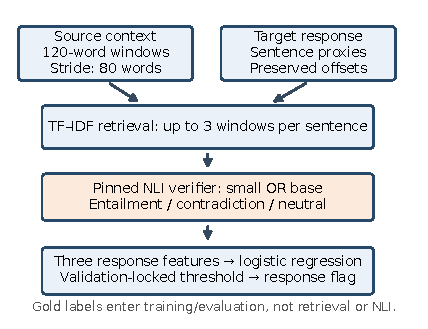
\includegraphics[width=\columnwidth]{figures/pipeline_original.pdf}
\caption{Original schematic of the evidence-only detector. The verifier checkpoint changes between systems; evidence windows and downstream training protocol are held fixed. Source text and target responses enter retrieval and verification, while gold labels enter only classifier training and evaluation.}
\label{fig:pipeline}
\end{figure}
\subsection{Sentence Proxies and Retrieval}
Responses are split by a deterministic punctuation/newline regular expression that preserves character offsets. These units can contain multiple claims or lose contextual qualifiers; we call them sentence proxies. Source context is split into overlapping 120-word windows with stride 80. For each response, a TF--IDF vectorizer is fitted to its source windows and sentence proxies without labels. Cosine-equivalent normalized dot products rank windows; stable sorting retains up to three per sentence. There is no web retrieval.

For QA, evidence consists of supplied passages, with the question excluded from NLI premises. Summaries use their source text. Data2txt inputs are recursively flattened with field names and values preserved. Changing the verifier does not rerun or alter these retrieval decisions.

\subsection{Verification and Response Features}
For sentence $s_j$ and retrieved window $e_{jk}$, NLI produces contradiction, entailment, and neutral probabilities. Define
\begin{align}
u_j &= 1-\max_k q_{jk}^{\mathrm{ent}},\label{eq:unsupported}\\
v_j &= \max_k q_{jk}^{\mathrm{con}},\label{eq:contradiction}\\
\mathbf{x}(y)&=\left[\max_j u_j,\ \max_j v_j,\ \frac{1}{m}\sum_{j=1}^{m}u_j\right].\label{eq:features}
\end{align}
Equations~\eqref{eq:unsupported}--\eqref{eq:features} define the implemented aggregation rules, rather than a new probabilistic theorem. Maximum entailment and contradiction can come from different windows. Consequently, these aggregates need not form one coherent evidence judgment. In particular, $u_j$ combines neutral and contradictory outcomes rather than separating insufficient retrieval from factual error.

A logistic regression with random seed 42 maps $\mathbf{x}(y)$ to a response score using the standard logistic link~\cite{sklearnlr}:
\begin{equation}
\widehat{p}(y)=\left[1+\exp\left(-b-\boldsymbol{\beta}^{\top}\mathbf{x}(y)\right)\right]^{-1}.\label{eq:logistic}
\end{equation}
Equation~\eqref{eq:logistic} uses fitted coefficients $\boldsymbol{\beta}$ and intercept $b$. Training uses the saved scikit-learn default configuration for both checkpoints; no verifier fine-tuning or task-specific classifier is performed. NLI inference uses float32, batch size 16, four CPU threads, a 512-token maximum, and premise-only truncation. Observed truncation counts are recorded rather than inferred from window lengths. No post-hoc probability calibration is fitted.

\subsection{Reproducibility and Execution}
The dataset commit is \texttt{c103204b9ce28d6bbad859304bf30de72b8ed8fe}. The small and base checkpoint revisions are respectively \texttt{fa2804872c3b4bd748f38c0185cc85775361e735} and \texttt{6c749ce3425cd33b46d187e45b92bbf96ee12ec7}. Configuration hashes, dataset checksums, fitted coefficients, predictions, environments, and migration checks are retained with the experiment artifacts. The recorded dependency lock includes scikit-learn 1.9.1, PyTorch 2.14.1, and Transformers 5.19.0.

Inference began on Windows CPU and continued on native Apple Silicon CPU. Limited migration checks found maximum NLI-probability differences of $5.48\times10^{-6}$ for the original checkpoint and $2.11\times10^{-6}$ for the alternative, below the recorded $10^{-4}$ continuation tolerance. These checks do not establish bitwise identity. Model inference is complete; saved predictions, rather than live progress counters, determine the reported sample counts.

\section{Results}
\subsection{Validation and Historical Operating Point}
At its historical threshold 0.29, the small detector obtains test precision 0.3772, recall 0.9139, and F1 0.5340, with 1,349 false positives and 77 false negatives. Its high detection rate therefore comes with many false alarms. Raising a threshold after viewing test errors would not be a valid improvement experiment.

Under the separate validation matched-recall rule, small/base precision is 0.4869/0.5075, with 1,176/1,084 false positives. Validation AUROC is 0.6422/0.6917 and AP is 0.5287/0.5789. Brier score improves from 0.2286 to 0.2189, while ECE worsens from 0.0293 to 0.0364. These validation results motivated freezing the base alternative for the test comparison; they are not independent evidence of generalization.

\subsection{Frozen Test Comparison}
Table~\ref{tab:test} reports the same 2,675 responses for both models. The base checkpoint has 0.0253 higher precision and 103 fewer false positives, an 8.2\% reduction relative to 1,256. Its achieved recall is 0.8915 versus 0.8736; neither necessarily equals the validation target. No recall noninferiority margin was prespecified for this completed comparison, so a formal recall-retention conclusion is not warranted.

% Original table from audited local results; no external table reuse.
\begin{table}[t]
\caption{Frozen test results. Differences are base minus small; intervals are archived conditional percentile summaries, not validated simultaneous coverage guarantees.}
\label{tab:test}\centering\footnotesize
\begin{tabular}{lrrl}\toprule
Metric & Small & Base & Descriptive 95\% interval\\\midrule
Precision & .3834 & .4087 & [.0140, .0367]\\
Recall & .8736 & .8915 & [$-$.0066, .0425]\\
F1 & .5329 & .5605 & [.0139, .0414]\\
AUROC & .6426 & .7016 & [.0384, .0807]\\
AP & .4257 & .4847 & [.0334, .0845]\\
Brier & .2137 & .2019 & [$-$.0161, $-$.0074]\\
ECE & .0631 & .0569 & [$-$.0136, .0075]\\\midrule
TP / FP & 781 / 1256 & 797 / 1153 & ---\\
TN / FN & 525 / 113 & 628 / 97 & ---\\\bottomrule
\end{tabular}
\end{table}


Ranking improves in the pooled sample: AUROC increases by 0.0589 and AP by 0.0590. Base AP is approximately 1.45 times test prevalence, compared with 1.27 for small. Nonetheless, base precision remains below 0.41 at this operating point; most flagged responses are negative under the operational labels. Figure~\ref{fig:diagnostics} presents precision--recall, reliability, and selective-acceptance diagnostics. The curves are post-hoc descriptions of frozen predictions and were not used to select new thresholds.

Figure~\ref{fig:confusion} visualizes the measured confusion counts on a common color scale. The alternative reduces false positives overall, but 1,153 false alarms remain.
\begin{figure}[t]
\centering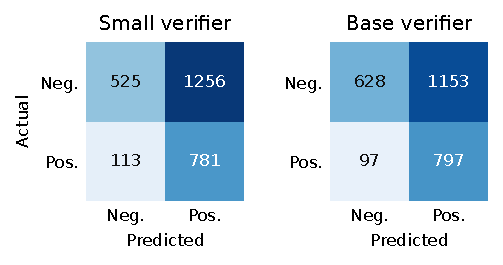
\includegraphics[width=\columnwidth]{figures/confusion_original.pdf}
\caption{Original confusion-matrix plots from the 2,675 frozen test predictions. Rows denote actual labels; columns denote predictions at each model's locked threshold. Color scales are identical.}
\label{fig:confusion}
\end{figure}

\begin{figure*}[t]
\centering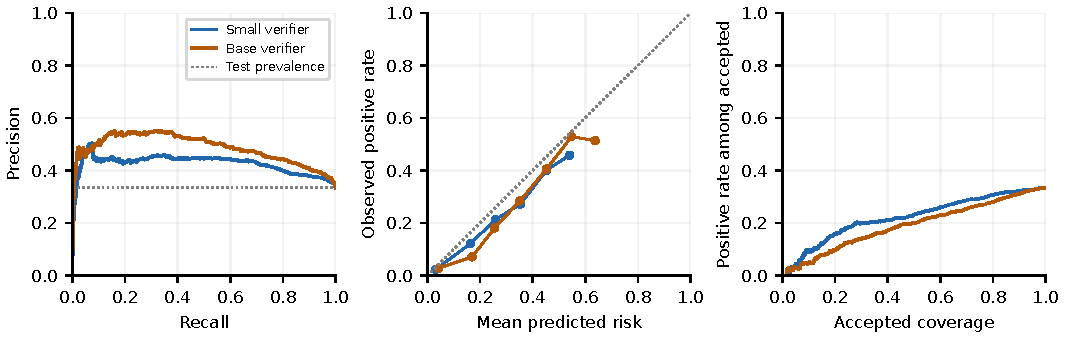
\includegraphics[width=\textwidth]{figures/verifier_diagnostics.pdf}
\caption{Diagnostics from the same frozen test predictions. Left: precision--recall curves with prevalence reference. Center: ten-bin reliability curves, displaying nonempty bins. Right: positive-label rate among responses accepted in ascending predicted-risk order; ties follow the saved response order. Selective risk here is not classification error. These are descriptive plots, not additional calibration training or confirmation experiments.}
\label{fig:diagnostics}
\end{figure*}

\subsection{Task-Stratified Findings}
Table~\ref{tab:tasks} is a post-hoc analysis using the same global locked thresholds. Positive prevalence ranges from 0.1531 in QA to 0.6267 in Data2txt. Higher Data2txt precision cannot therefore be interpreted as intrinsically superior detection. All tasks have higher base AUROC and AP, but operational effects differ. Summary gains precision while recall falls from 0.8112 to 0.7908. Data2txt gains recall but adds eight false positives (278 to 286). Pooled recall improvement does not establish retention within every task, and pooled calibration can hide large task-specific errors.

Figure~\ref{fig:task-tradeoffs} makes these distinct precision--recall trade-offs visible. No task-specific threshold tuning is performed.
\begin{figure}[t]
\centering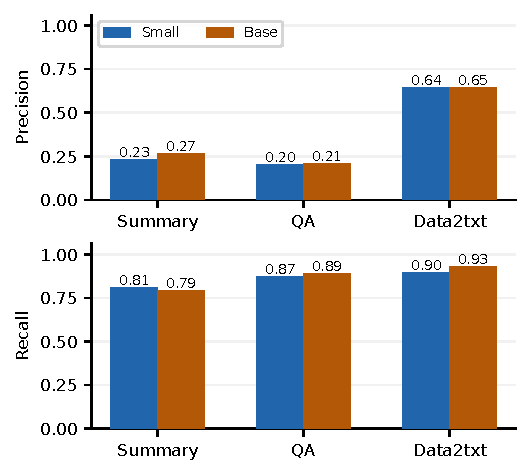
\includegraphics[width=\columnwidth]{figures/task_tradeoffs_original.pdf}
\caption{Original task-level plots from saved test results, at unchanged global thresholds. Both vertical axes start at zero. Labels are rounded to two decimal places; Table~\ref{tab:tasks} gives higher precision. These are descriptive point estimates without invented error bars.}
\label{fig:task-tradeoffs}
\end{figure}

% Original table from audited local results; no external table reuse.
\begin{table}[t]
\caption{Post-hoc task results at unchanged global thresholds. Each row contains small/base values; all tasks have 150 test sources.}
\label{tab:tasks}\centering\footnotesize
\begin{tabular}{lrrr}\toprule
 & Summary & QA & Data2txt\\\midrule
Responses & 900 & 875 & 900\\
Prevalence & .2178 & .1531 & .6267\\
Precision & .2345/.2677 & .2031/.2117 & .6450/.6465\\
Recall & .8112/.7908 & .8731/.8881 & .8954/.9273\\
AUROC & .6025/.6472 & .6731/.7035 & .6206/.6356\\
AP & .2897/.3218 & .2207/.2483 & .7229/.7293\\\bottomrule
\end{tabular}
\end{table}


\subsection{Source-Overlap Sensitivity}\label{sec:overlap}
Later audits identified two exact QA-passage relationships spanning historical training and test folds, affecting 12 test responses. Another exact Summary-content pair spans training and validation. A broader deterministic scan of 2,965 source records found 66 pairs sharing at least 40 contiguous normalized words, with 29 pairs crossing historical folds. These are verified shared-text flags, not an exhaustive semantic-duplicate audit or proof of performance bias.

We form conservative connected components from these flagged edges and the previously recorded related-source edges. As a post-hoc sensitivity check, test sources connected to any official-training source are excluded. The check removes 12 test sources and 72 responses, leaving 2,603 responses from 438 source IDs. Models, scores, and thresholds are unchanged; this is not a newly collected test set, retraining experiment, or claim of complete independence.

% Original table from audited local results; no external table reuse.
\begin{table}[t]
\caption{Post-hoc exclusion sensitivity; small/base values. No thresholds are reselected.}
\label{tab:sensitivity}\centering\footnotesize
\begin{tabular}{lrrr}\toprule
Test subset & $N$ & Precision & AUROC\\\midrule
Original & 2675 & .3834/.4087 & .6426/.7016\\
Remove two QA sources & 2663 & .3837/.4090 & .6432/.7009\\
Remove flagged components & 2603 & .3859/.4110 & .6450/.7026\\\bottomrule
\end{tabular}
\end{table}


The precision difference remains approximately 0.0251 after the broader exclusion, with recall 0.8727/0.8899 and AP 0.4282/0.4864. This suggests that the observed point-estimate pattern is not confined to the identified test-linked records. It does not undo training--validation overlap, detect unflagged dependencies, or validate the original source-bootstrap assumptions.

\subsection{Error Diagnosis and Computational Cost}
An exploratory review sampled 100 validation false positives and 50 validation false negatives. One assistant assigned provisional primary categories, preserving original working diagnoses; no independent human error-category validation or gold relabeling was performed. Among reviewed false positives, verification (30), context/attribution (29), segmentation (20), and retrieval (15) dominated. The sample was stratified, so these counts are not estimated population cause frequencies. False-negative notes included unsupported/contradicted claims (22) and verification errors (14); the former describes the evidence relationship rather than a causal mechanism.

The historical small-detector sentence-overlap proxy achieves test precision 0.1070, recall 0.7056, and F1 0.1858 at its validation-selected sentence threshold. This weak localization reinforces that response-level gains do not establish atomic-claim or exact-span detection quality.

The original all-fold inference record contains 389,371 NLI pairs, zero observed truncations, and 33,019.57 cumulative seconds across Windows and Mac CPU execution. The alternative test continuation records 56,317 newly computed pairs, zero truncations, and 4,118.21 cumulative inference seconds. Pair caches affect newly computed work. These scopes and hardware histories differ, so neither a relative speedup nor a controlled cost--accuracy advantage can be inferred.

\section{Discussion and Limitations}
The controlled comparison supports using the base checkpoint as an evidence-only reference in subsequent research, but not unqualified deployment. Precision remains low, summary recall decreases, and the benchmark's task mixture influences pooled results. Treating all unentailed text as hallucinated can conflate missing evidence with contradiction. Retrieval, segmentation, window aggregation, and label interpretation remain plausible error sources that a larger checkpoint alone cannot eliminate.

Our study compares only two checkpoints and one shallow aggregation design. It does not establish superiority over specialized hallucination detectors, include a retrieval/segmentation ablation, or measure generalization to unseen generator families or new domains. Fixed test examples have now been inspected; future model selection must use development data and future confirmation needs an appropriately independent source frame.

The operational labels are derived from existing RAGTruth annotations, not newly validated factuality judgments. Excluding incorrect refusals and truncated responses narrows the population. A response-level positive label ignores hallucination extent, and sentence proxies can overlap spans without isolating the factual error. Assistant-generated silver-label pilots and statistical-engineering simulations from the broader project are not evidence for the detector results reported here.

\method's intended consistency-plus-evidence comparison remains unresolved. A valid extension requires controlled same-generator sampling, labels for the actual target responses, matched evaluation examples, and a justified inference procedure. Repeated agreement is not proof of factuality. Software tests and optimizer certification, including later repairs, do not substitute for that effectiveness experiment.

\section{Conclusion}
Replacing the small NLI verifier with the base checkpoint in a fixed evidence-only pipeline improves pooled test precision by 2.53 percentage points and AUROC by 0.0589, with 103 fewer false positives at independently validation-selected high-recall operating points. Task analysis reveals a summary-recall decrease and minimal Data2txt precision change. Post-hoc shared-content exclusions preserve a similar precision difference but do not establish full source independence. These results provide an auditable evidence-verification reference with explicit failure modes; whether self-consistency adds useful information remains an open empirical question.

\section*{Reproducibility and Data Availability}
The project repository is \href{https://github.com/algorithmist-yash/EviConsist}{github.com/algorithmist-yash/EviConsist}~\cite{repository}. It provides the implementation, manuscript source, original figure-generation code, configuration records, and aggregate result tables. Response-level prediction archives and raw corpus text remain local. The accompanying analysis script recomputes the reported point estimates and plots from those saved predictions without retraining or threshold tuning; regenerating prediction-level curves requires those local artifacts. Upstream article, passage, and review rights are not inferred from repository licensing, and raw source text is not redistributed. Provider/release provenance remains an acknowledged limitation.

\section*{Acknowledgment}
OpenAI Codex assisted with implementation, exploratory error analysis, analysis and plotting code, and manuscript drafting and revision. Assistant-generated reviews are provisional, not independent human annotations. Detector labels use the benchmark annotations under the stated mapping.

\begin{thebibliography}{00}
\bibitem{lewisrag} P.~Lewis \emph{et al.}, ``\href{https://arxiv.org/abs/2005.11401}{Retrieval-augmented generation for knowledge-intensive NLP tasks},'' in \emph{Proc. NeurIPS}, 2020. [Online]. Available: \url{https://arxiv.org/abs/2005.11401}
\bibitem{ragtruth} C.~Niu \emph{et al.}, ``\href{https://aclanthology.org/2024.acl-long.585/}{RAGTruth: A hallucination corpus for developing trustworthy retrieval-augmented language models},'' in \emph{Proc. ACL}, 2024, pp.~10862--10878, doi: \href{https://doi.org/10.18653/v1/2024.acl-long.585}{10.18653/v1/2024.acl-long.585}.
\bibitem{maynez} J.~Maynez, S.~Narayan, B.~Bohnet, and R.~McDonald, ``\href{https://aclanthology.org/2020.acl-main.173/}{On faithfulness and factuality in abstractive summarization},'' in \emph{Proc. ACL}, 2020, pp.~1906--1919, doi: \href{https://doi.org/10.18653/v1/2020.acl-main.173}{10.18653/v1/2020.acl-main.173}.
\bibitem{halueval} J.~Li, X.~Cheng, W.~X.~Zhao, J.-Y.~Nie, and J.-R.~Wen, ``\href{https://aclanthology.org/2023.emnlp-main.397/}{HaluEval: A large-scale hallucination evaluation benchmark for large language models},'' in \emph{Proc. EMNLP}, 2023, pp.~6449--6464, doi: \href{https://doi.org/10.18653/v1/2023.emnlp-main.397}{10.18653/v1/2023.emnlp-main.397}.
\bibitem{fever} J.~Thorne, A.~Vlachos, C.~Christodoulopoulos, and A.~Mittal, ``\href{https://aclanthology.org/N18-1074/}{FEVER: A large-scale dataset for fact extraction and verification},'' in \emph{Proc. NAACL-HLT}, 2018, pp.~809--819, doi: \href{https://doi.org/10.18653/v1/N18-1074}{10.18653/v1/N18-1074}.
\bibitem{scifact} D.~Wadden \emph{et al.}, ``\href{https://aclanthology.org/2020.emnlp-main.609/}{Fact or fiction: Verifying scientific claims},'' in \emph{Proc. EMNLP}, 2020, pp.~7534--7550, doi: \href{https://doi.org/10.18653/v1/2020.emnlp-main.609}{10.18653/v1/2020.emnlp-main.609}.
\bibitem{frank} A.~Pagnoni, V.~Balachandran, and Y.~Tsvetkov, ``\href{https://aclanthology.org/2021.naacl-main.383/}{Understanding factuality in abstractive summarization with FRANK: A benchmark for factuality metrics},'' in \emph{Proc. NAACL-HLT}, 2021, pp.~4812--4829, doi: \href{https://doi.org/10.18653/v1/2021.naacl-main.383}{10.18653/v1/2021.naacl-main.383}.
\bibitem{truebenchmark} O.~Honovich \emph{et al.}, ``\href{https://aclanthology.org/2022.dialdoc-1.19/}{TRUE: Re-evaluating factual consistency evaluation},'' in \emph{Proc. Second DialDoc Workshop}, 2022, pp.~161--175, doi: \href{https://doi.org/10.18653/v1/2022.dialdoc-1.19}{10.18653/v1/2022.dialdoc-1.19}.
\bibitem{factscore} S.~Min \emph{et al.}, ``\href{https://arxiv.org/abs/2305.14251}{FActScore: Fine-grained atomic evaluation of factual precision in long form text generation},'' arXiv:2305.14251, 2023, doi: \href{https://doi.org/10.48550/arXiv.2305.14251}{10.48550/arXiv.2305.14251}.
\bibitem{alignscore} Y.~Zha, Y.~Yang, R.~Li, and Z.~Hu, ``\href{https://aclanthology.org/2023.acl-long.634/}{AlignScore: Evaluating factual consistency with a unified alignment function},'' in \emph{Proc. ACL}, 2023, pp.~11328--11348, doi: \href{https://doi.org/10.18653/v1/2023.acl-long.634}{10.18653/v1/2023.acl-long.634}.
\bibitem{smallcard} Sentence Transformers, ``cross-encoder/nli-deberta-v3-small,'' model card, accessed Nov.~1, 2026. [Online]. Available: \url{https://huggingface.co/cross-encoder/nli-deberta-v3-small}
\bibitem{basecard} Sentence Transformers, ``cross-encoder/nli-deberta-v3-base,'' model card, accessed Nov.~1, 2026. [Online]. Available: \url{https://huggingface.co/cross-encoder/nli-deberta-v3-base}
\bibitem{factcc} W.~Kryscinski, B.~McCann, C.~Xiong, and R.~Socher, ``\href{https://aclanthology.org/2020.emnlp-main.750/}{Evaluating the factual consistency of abstractive text summarization},'' in \emph{Proc. EMNLP}, 2020, pp.~9332--9346, doi: \href{https://doi.org/10.18653/v1/2020.emnlp-main.750}{10.18653/v1/2020.emnlp-main.750}.
\bibitem{summac} P.~Laban, T.~Schnabel, P.~N.~Bennett, and M.~A.~Hearst, ``\href{https://aclanthology.org/2022.tacl-1.10/}{SummaC: Re-visiting NLI-based models for inconsistency detection in summarization},'' \emph{Trans. Assoc. Comput. Linguistics}, vol.~10, pp.~163--177, 2022, doi: \href{https://doi.org/10.1162/tacl_a_00453}{10.1162/tacl\_a\_00453}.
\bibitem{qags} A.~Wang, K.~Cho, and M.~Lewis, ``\href{https://aclanthology.org/2020.acl-main.450/}{Asking and answering questions to evaluate the factual consistency of summaries},'' in \emph{Proc. ACL}, 2020, pp.~5008--5020, doi: \href{https://doi.org/10.18653/v1/2020.acl-main.450}{10.18653/v1/2020.acl-main.450}.
\bibitem{qafacteval} A.~Fabbri, C.-S.~Wu, W.~Liu, and C.~Xiong, ``\href{https://aclanthology.org/2022.naacl-main.187/}{QAFactEval: Improved QA-based factual consistency evaluation for summarization},'' in \emph{Proc. NAACL-HLT}, 2022, pp.~2587--2601, doi: \href{https://doi.org/10.18653/v1/2022.naacl-main.187}{10.18653/v1/2022.naacl-main.187}.
\bibitem{snli} S.~R.~Bowman, G.~Angeli, C.~Potts, and C.~D.~Manning, ``\href{https://aclanthology.org/D15-1075/}{A large annotated corpus for learning natural language inference},'' in \emph{Proc. EMNLP}, 2015, pp.~632--642, doi: \href{https://doi.org/10.18653/v1/D15-1075}{10.18653/v1/D15-1075}.
\bibitem{multinli} A.~Williams, N.~Nangia, and S.~R.~Bowman, ``\href{https://aclanthology.org/N18-1101/}{A broad-coverage challenge corpus for sentence understanding through inference},'' in \emph{Proc. NAACL-HLT}, 2018, pp.~1112--1122, doi: \href{https://doi.org/10.18653/v1/N18-1101}{10.18653/v1/N18-1101}.
\bibitem{debertav3} P.~He, J.~Gao, and W.~Chen, ``\href{https://arxiv.org/abs/2111.09543}{DeBERTaV3: Improving DeBERTa using ELECTRA-style pre-training with gradient-disentangled embedding sharing},'' in \emph{Proc. ICLR}, 2023. [Online]. Available: \url{https://arxiv.org/abs/2111.09543}
\bibitem{selfcheck} P.~Manakul, A.~Liusie, and M.~J.~F.~Gales, ``\href{https://aclanthology.org/2023.emnlp-main.557/}{SelfCheckGPT: Zero-resource black-box hallucination detection for generative large language models},'' in \emph{Proc. EMNLP}, 2023, pp.~9004--9017, doi: \href{https://doi.org/10.18653/v1/2023.emnlp-main.557}{10.18653/v1/2023.emnlp-main.557}.
\bibitem{semanticentropy} S.~Farquhar, J.~Kossen, L.~Kuhn, and Y.~Gal, ``\href{https://www.nature.com/articles/s41586-024-07421-0}{Detecting hallucinations in large language models using semantic entropy},'' \emph{Nature}, vol.~630, pp.~625--630, 2024, doi: \href{https://doi.org/10.1038/s41586-024-07421-0}{10.1038/s41586-024-07421-0}.
\bibitem{sklearnmetrics} scikit-learn developers, ``\href{https://scikit-learn.org/stable/modules/model_evaluation.html}{Metrics and scoring: Quantifying the quality of predictions},'' scikit-learn documentation, accessed Nov.~1, 2026. [Online]. Available: \url{https://scikit-learn.org/stable/modules/model_evaluation.html}
\bibitem{guocalibration} C.~Guo, G.~Pleiss, Y.~Sun, and K.~Q.~Weinberger, ``\href{https://proceedings.mlr.press/v70/guo17a.html}{On calibration of modern neural networks},'' in \emph{Proc. ICML}, vol.~70, 2017, pp.~1321--1330.
\bibitem{sklearnlr} scikit-learn developers, ``\href{https://scikit-learn.org/stable/modules/generated/sklearn.linear_model.LogisticRegression.html}{LogisticRegression},'' scikit-learn documentation, accessed Nov.~1, 2026. [Online]. Available: \url{https://scikit-learn.org/stable/modules/generated/sklearn.linear_model.LogisticRegression.html}
\bibitem{repository} S.~Ranjan, Y.~Raj, S.~Singh, S.~Srivastava, and S.~Bajoria, ``\href{https://github.com/algorithmist-yash/EviConsist}{EviConsist: Evidence verification for hallucination detection},'' project source repository, 2026. [Online]. Available: \url{https://github.com/algorithmist-yash/EviConsist}
\end{thebibliography}
\end{document}
